\documentclass{article} % A4 paper and 11pt font size
\setcounter{secnumdepth}{0}

\usepackage{amssymb, amsmath, amsfonts}
\usepackage{moreverb}
\usepackage{graphicx}
\usepackage{subcaption}
\usepackage{extarrows}
\usepackage{enumerate}
\usepackage{graphics}
\usepackage[margin=1.25in]{geometry}
\usepackage{color}
\usepackage{tocloft}
\renewcommand{\cftsecleader}{\cftdotfill{\cftdotsep}}
\usepackage{array}
\usepackage{float}
\usepackage{hyperref}
\usepackage{textcomp}
\usepackage[makeroom]{cancel}
\usepackage{bbold}
\usepackage{alltt}
\usepackage{physics}
\usepackage{mathtools}
\usepackage[normalem]{ulem}
\usepackage{amsthm}
\usepackage{tikz}
\usetikzlibrary{positioning}
\usetikzlibrary{arrows}
\usepackage{pgfplots}
\usepackage{bigints}
\allowdisplaybreaks
\pgfplotsset{compat=1.12}

\theoremstyle{plain}
\newtheorem*{theorem*}{Theorem}
\newtheorem{theorem}{Theorem}
\newtheorem*{lemma*}{Lemma}
\newtheorem{lemma}{Lemma}

\newenvironment{definition}[1][Definition]{\begin{trivlist}
\item[\hskip \labelsep {\bfseries #1}]}{\end{trivlist}}

\newcommand{\E}{\varepsilon}
\def\Rl{\mathbb{R}}
\def\Cx{\mathbb{C}}

\usepackage[T1]{fontenc} % Use 8-bit encoding that has 256 glyphs
\usepackage{fourier} % Use the Adobe Utopia font for the document - comment this line to return to the LaTeX default
\usepackage[english]{babel} % English language/hyphenation

\usepackage{sectsty} % Allows customizing section commands
\allsectionsfont{\centering \normalfont\scshape} % Make all sections centered, the default font and small caps

\usepackage{fancyhdr} % Custom headers and footers
\pagestyle{fancy} % Makes all pages in the document conform to the custom headers and footers
\fancyhead[L]{\bf Sam Fleischer}
\fancyhead[C]{\bf UC Davis \\ Analysis (MAT280)} % No page header - if you want one, create it in the same way as the footers below
\fancyhead[R]{\bf Spring 2016}

\fancyfoot[L]{\bf } % Empty left footer
\fancyfoot[C]{\bf \thepage} % Empty center footer
\fancyfoot[R]{\bf } % Page numbering for right footer
\renewcommand{\headrulewidth}{0pt} % Remove header underlines
\renewcommand{\footrulewidth}{0pt} % Remove footer underlines
\setlength{\headheight}{25pt} % Customize the height of the header

\newcommand{\VEC}[2]{\left\langle #1, #2 \right\rangle}
\newcommand{\ran}{\text{\rm ran }}
\newcommand{\Hilb}{\mathcal{H}}

\DeclareMathOperator*{\esssup}{\text{ess~sup}}

\newcommand{\problem}[2]{
\vspace{.375cm}
\boxed{\begin{minipage}{\textwidth}
    \section*{\bf #1}
    #2
\end{minipage}}
}

\numberwithin{equation}{section} % Number equations within sections (i.e. 1.1, 1.2, 2.1, 2.2 instead of 1, 2, 3, 4)
\numberwithin{figure}{section} % Number figures within sections (i.e. 1.1, 1.2, 2.1, 2.2 instead of 1, 2, 3, 4)
\numberwithin{table}{section} % Number tables within sections (i.e. 1.1, 1.2, 2.1, 2.2 instead of 1, 2, 3, 4)

\setlength\parindent{0pt} % Removes all indentation from paragraphs - comment this line for an assignment with lots of text

\newcommand{\horrule}[1]{\rule{\linewidth}{#1}} % Create horizontal rule command with 1 argument of height

\usepackage{xcolor}
\definecolor{light-gray}{gray}{0.9}

\title{ 
\normalfont \normalsize 
\textsc{UC Davis, Big Data (MAT280), Spring 2016} \\ [25pt] % Your university, school and/or department name(s)
\horrule{2pt} \\[0.4cm] % Thin top horizontal rule
\Huge Homework \#1 \\ % The assignment title
\horrule{2pt} \\[0.5cm] % Thick bottom horizontal rule
}

\author{\huge Sam Fleischer} % Your name

\date{April 18, 2016} % Today's date or a custom date

\begin{document}\thispagestyle{empty}

\maketitle % Print the title

\makeatletter
\@starttoc{toc}
\makeatother

\pagebreak

%%%%%%%%%%%%%%%%%%%%%%%%%%%%%%%%%%%%%%
\problem{Problem 1}{Show that two random vectors in high dimensions are almost orthogonal. \\

\emph{Note: In your theorem you need to formalize what ``almost orthogonal'' means (what it means will come out of your proof ). You first need to select a probability distribution of your choice and apply an appropriate concentration inequality (but keep in mind that if e.g.~$x$ and $y$ are Gaussian random vectors, then the entries of the inner product $\VEC{x}{y}$ are no longer Gaussian).}}
\begin{proof}
    Let $a$ be a uniformly chosen random vector on the unit sphere in $\Rl^d$.  Now let $a$ be the first element of an orthonormal basis $\{a\}$ and extend this, via Gram-Schmidt, to an orthonormal basis of $\Rl^d$: $B = \{a, a_1, \dots, a_{d-1}\}$.  In polar coordinates,
    \begin{align*}
        a = \qty(1, \frac{\pi}{2}, \frac{\pi}{2}, \dots, \frac{\pi}{2}, \frac{\pi}{2})
    \end{align*}
    where the first entry is magnitude $\rho$, the last entry $\theta \in [0, 2\pi)$, and all other entries $\phi_i \in [0, \pi)$ for $i = 1, \dots, d-2$.  These coordinates are essentally a rotation such that $a$ is parallel with the positive $x$-axis.  In rectangular coordinates,
    \begin{align*}
        a = (0, 0, \dots, 0, 1)
    \end{align*}
    which represents the components of the basis $B$ of $\Rl^n$.  Now let $b$ be chosen uniformly at random on the unit sphere.  That is, $\norm{b} = 1$ and $\theta \in [0,2\pi)$ is chosen uniformly at random and $\phi_1, \dots, \phi_{d-2} \in [0, \pi)$ are each chosen uniformly at random.  $b$ can be represented in the polar coordinates as defined above as
    \begin{align*}
        b = \qty(1, \phi_1, \phi_2, \dots, \phi_{d-2}, \theta)
    \end{align*}
    and in rectangular coordinates as
    \begin{align*}
        b = \qty(b_1, b_2, \dots, b_d)
    \end{align*}
    where
    \begin{align*}
        b_1 &= \cos(\phi_1) \\
        b_2 &= \sin(\phi_1)\cos(\phi_2) \\
        b_3 &= \sin(\phi_1)\sin(\phi_2)\cos(\phi_3) \\
        \vdots\ \ & \\
        b_{d-2} &= \sin(\phi_1)\sin(\phi_2)\sin(\phi_3)\dots\sin(\phi_{d-3})\cos(\phi_{d-2})\\
        b_{d-1} &= \sin(\phi_1)\sin(\phi_2)\sin(\phi_3)\dots\sin(\phi_{d-3})\sin(\phi_{d-2})\cos(\theta) \\
        b_d &= \sin(\phi_1)\sin(\phi_2)\sin(\phi_3)\dots\sin(\phi_{d-3})\sin(\phi_{d-2})\sin(\theta)
    \end{align*}
    Then
    \begin{align*}
        \VEC{a}{b} = \VEC{(0, 0, \dots, 0, 1)}{\qty(b_1, b_2, \dots, b_d)} = b_d = \sin(\phi_1)\sin(\phi_2)\sin(\phi_3)\dots\sin(\phi_{d-3})\sin(\phi_{d-2})\sin(\theta).
    \end{align*}
    This is a product of $d-1$ numbers in $[-1,1]$.  Note that since $\phi_1, \dots, \phi_{d-2}$ are independent indentical random variables uniformly distributed in $[0,\pi)$, and since $\theta$ is uniformly distributed in $[0,2\pi)$ then
    \begin{align*}
        \mathbb{P}\qty(\abs{\sin(\phi_i)} > \frac{1}{2}) = \frac{2}{3} \qquad \text{and} \qquad \mathbb{P}\qty(\abs{\sin(\theta)} > \frac{1}{2}) = \frac{2}{3}
    \end{align*}
    Thus,
    \begin{align*}
        \mathbb{P}\qty(\VEC{a}{b} > \frac{1}{2^{d-1}}) = \mathbb{P}\qty(\abs{\sin(\theta)\prod_{i=1}^{d-2}\sin(\phi_{i})} > \frac{1}{2^{d-1}}) = \qty(\frac{2}{3})^{d-1} \rightarrow 0 \qquad \text{as } d \rightarrow \infty
    \end{align*}
    Thus two random vectors in high dimensions are most likely orthogonal.
\end{proof}







%%%%%%%%%%%%%%%%%%%%%%%%%%%%%%%%%%%%%%
\problem{Problem 2}{Consider the following setup.  Given a square of side length 1, we place four circles in the square as depicted in Figure~\ref{fig1} (each of the gray circles has radius 1/4).  We now place a circle at the center of the square (the blue circle in Figure~\ref{fig1}) such that this circle in the middle touches each of the four identical circles. Let $r$ denote the radius of the blue circle. \\

We can do something analogous in three dimensions, see Figure~\ref{fig2}.  We place eight spheres of radius 1/4 inside a cube of side length 1, and put a (blue) sphere in the middle such that it touches all eight (gray) spheres. \\

In four dimensions we can arrange 16 hyperspheres of radius 1/4 inside a hypercube of side length 1 and place a hypersphere in the middle, so that this hypersphere all the other 16 hyperspheres. \\

Obviously we can do this for increasing dimension $d$.  What happens with the blue hypersphere in the middle as $d$ increases?  Will it shrink?  Will it be of constant size?  Will it grow outside the hypercube? \\

(Hint: Check the diameter of the blue hypersphere in comparison to the sidelength of the cube as $d$ increases.  This is actually not difficult to compute, it may sound more complicated than it is).
}

\begin{figure}[ht!]
\centering
\begin{subfigure}{.5\textwidth}
    \centering
    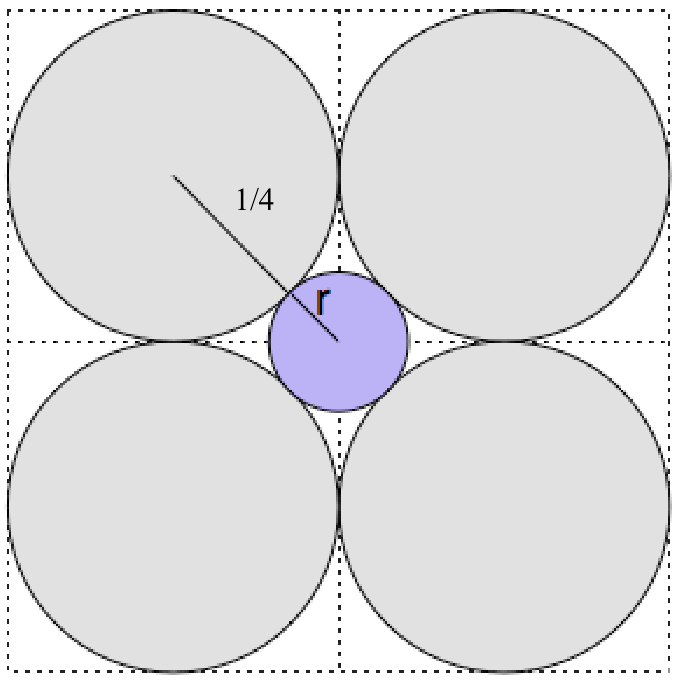
\includegraphics[width=40mm]{figures/4circles1}
    \caption{4 circles}
    \label{fig1}
\end{subfigure}%
\begin{subfigure}{.5\textwidth}
    \centering
    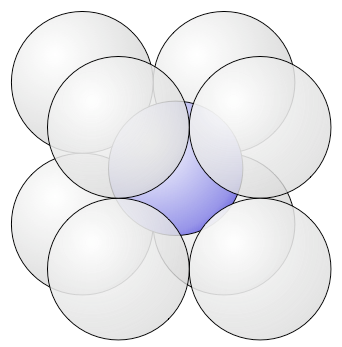
\includegraphics[width=40mm]{figures/8spheres}
    \caption{8 spheres}
    \label{fig2}
\end{subfigure}
\caption{}
\label{fig:test}
\end{figure}

\begin{proof}
    In a given orthant, the hypersphere of radius $\frac{1}{4}$ is always tangent to the hypercube of apothem size $\frac{1}{4}$.  However, the distance from each vertex of the hypercube of apothem size $\frac{1}{4}$ to the center that hypercube is $\frac{\sqrt{d}}{4}$.  The origin (center of the blue hypersphere) is a vertex of each orthant's hypercube, and thus the radius of the blue sphere is at most $\frac{1 - \sqrt{d}}{4}$.  A worse upper bound is the distance from the origin to the point at which two hyperspheres meet, which is $\frac{\sqrt{d-1}}{4}$.  Since two hyperspheres can only meet at one point, they must meet when the blue hypersphere has radius
    \begin{align*}
        r_{\text{blue hypersphere}} = \frac{1 - \sqrt{d}}{4}.
    \end{align*}
\end{proof}








%%%%%%%%%%%%%%%%%%%%%%%%%%%%%%%%%%%%%%
\problem{Problem 3}{Show that for every fixed dimension reduction matrix $A$ of size $k \times d$ with $k < d$, there exists vectors $x,y \in \Rl^d$ such that the distance  $\norm{Ax-Ay}$ (no matter which norm we use) is vastly different from $\norm{x-y}$.}
\begin{proof}
    First note that $\dim \ran A \leq k < d$.  Thus, by the Fundamental Theorem of Linear Algebra, $\dim \text{null} A \geq 1$.  Then let $x \in \text{null} A$ and let $y = ax$.  Thus $y \in \text{null} A$ and $\norm{x - y} \rightarrow \infty$ as $a \rightarrow \infty$.  However $\norm{Ax - Ay} = \norm{0 - 0} = 0$ for all values of $a$.
\end{proof}








%%%%%%%%%%%%%%%%%%%%%%%%%%%%%%%%%%%%%%
\problem{Problem 4}{The Yale Face Database contains images from various individuals in different poses and under different lighting conditions.  Some of the images are stored in the file {\tt SomeYaleFaces.mat}. \\

Load this file into Matlab. The variable {\tt X} is a matrix of size $1024 \times 2414$. Each column of {\tt X} is an image of size $32 \times 32$ (in vectorized form).  The 2414 columns are images of 38 different persons in about 64 poses each.  You can easily covert the $k$-th column of {\tt X} back to an image via the commands \\
{\tt xk = X(:,k);} \\
{\tt xk = reshape(xk,32,32);} \\

The command \\ 
{\tt imagesc(x1); colormap(gray);} \\
will display the image. \\

You can conveniently display multiple images if you want with the file {\tt showfaces.m}. \\

We want to compare three dimension reduction methods by comparing how well distances between the different images are preserved: (i) Johnson-Lindenstrauss projection, Fast Johnson Lindenstrauss projection and simple random sampling (i.e., randomly picking $k$ indices). \\

Choose different values for the reduced dimension $k$ and compare the dimension reduction ability of the three methods.  You need to think about how to devise such an experiment.  There are of course multiple options to do so.}

\begin{proof}
    I first used three 
    \subsubsection*{Johnson-Lindenstrauss projection}
    \subsubsection*{Fast Johnson-Lindenstrauss projection}
    \subsubsection*{Simple random sampling}
\end{proof}









\end{document}
